% ---------------------------------------------------------------------------
% Preliminary appendix: full method x region x year grid.
% Place after Appendix D. Needs only multirow / pifont / graphicx (already in
% the preamble). Tables are generated -- do not hand-edit appendix_tables.tex:
%   python scripts/analysis/make_appendix_tables.py --out paper/appendix_tables.tex
% ---------------------------------------------------------------------------

\section{Extended Results: 33 Methods $\times$ 4 Regions $\times$ 2 Years}
\label{app:extended}

The main text reports year 2019 for a subset of the evaluated methods. This
appendix reports the complete re-run grid: all 33 methods in
Table~\ref{tab:app_coverage}, on all four LargeST subsets, for both 2018 and
2019. Beyond breadth it does three things the single-year tables cannot.
First, it adds two model families absent from the main text---deep state-space
models and linear forecasters---which turn out to occupy the gap between the
task-trained graph models and the pretrained forecasters. Second, the second
year converts the comparison into a replication: an ordering that survives both
years is a property of the method, whereas one that flips is a property of the
year. Third, it records which methods could not be run at all at scale, which
is itself a deployment result.

\subsection{Additional methods}
\label{app:extended:methods}

\textit{Deep state-space models (SSM).} Structured state-space sequence models
are task-trained, like the GNNs, but run per sensor series, like the foundation
models. That combination makes them the control this benchmark was missing: they
separate the contribution of the architecture class from the contribution of
large-scale pretraining, and they do so without a road graph. We evaluate a
minimal diagonal linear time-invariant model (\textbf{Linear SSM}),
\textbf{S4}~\citep{gu2022s4, gu2022s4d} with HiPPO-inspired initialization and a
learnable step size, the \textbf{LRU}~\citep{orvieto2023lru} with complex
eigenvalues and an output gate, and \textbf{Mamba-v2}~\citep{dao2024mamba2}, a
selective SSM with an input-dependent state transition. Each maps a length-$L$ univariate context to $H$ steps directly and
is trained under the same splits, normalization and early stopping as the GNNs.

\textit{Linear forecasters.} \textbf{DLinear} and \textbf{NLinear}~\citep{zeng2023transformers}
are single-layer linear maps from context to horizon---the former over a
trend/seasonal decomposition, the latter over a last-value-normalized input.
They were introduced as evidence that much of the reported gain from deep
forecasters is recoverable linearly, and as the cheapest trained methods here
they calibrate what the rest of the table buys.

\subsection{Coverage and failures at scale}
\label{app:extended:coverage}

Table~\ref{tab:app_coverage} records which methods ran on which subset. The
gaps are not incidental and they fall on one family: the $O(N^2)$ graph
operators exhaust GPU memory as the sensor count grows, so \textbf{STGODE} is
unavailable on every subset, \textbf{D2STGNN} beyond SD, and \textbf{DGCRN}
beyond SD and GBA~2018. These methods are kept as rows in every table, with
their entries shown as ``-'', so that the composition of each family stays
visible. This matters for reading the tables, because the
unavailable models are not arbitrary members of their family: \texttt{DGCRN}
records the lowest Avg MAE of any graph model on SD in both years (17.65 in 2019,
17.13 in 2018) and \texttt{D2STGNN} places third or fourth, yet neither can be
run on GLA or CA. The graph family's strongest member is therefore absent from
exactly the subsets where the forecasting problem is hardest, and the GLA and CA
columns compare the remainder. A missing cell means the run did not produce a usable result---never
that the method scored poorly.


\subsection{Results by region and year}
\label{app:extended:tables}

Tables~\ref{tab:app_sd_2019}--\ref{tab:app_ca_2018} give the grid, one table per
subset and year, in the column layout of the main text. Best per column is bold,
runner-up underlined; comparisons are within a table, never across them. A
``-'' marks a method that did not produce a usable result on that subset, not a
poor score.

FlowState is listed for completeness and is unavailable throughout. We discuss
each subset over both years in turn, then draw the comparison across regions.

\subsubsection{San Diego (716 sensors)}
\label{app:extended:sd}

SD is the smallest subset and the only one where the graph family is
competitive. \texttt{DGCRN} is the best graph model in both years (Avg MAE
17.13 in 2018, 17.65 in 2019) and in 2019 it beats every state-space model
(\texttt{LRU}, 18.41); in 2018 the order reverses by a small margin
(\texttt{LRU} 16.97 against \texttt{DGCRN} 17.13). At the shortest horizon the
gap to the pretrained models is narrow---\texttt{DGCRN} reaches 14.58 MAE at
$H{=}3$ in 2018 against \texttt{Sundial}'s 14.24---so on a network of this size
the spatial prior is close to paying for itself. It does not hold up as the
horizon extends: \texttt{DGCRN} degrades by a factor of $1.43$ from $H{=}3$ to
$H{=}12$ while \texttt{Sundial} is flat, and the full-grid ordering by Avg MAE
is \texttt{Sundial} $<$ \texttt{Moirai-2} $<$ \texttt{Chronos-Bolt} $<$
\texttt{Kairos} before any task-trained model appears.

\begin{insightbox}
\textit{Takeaway:} On the smallest network the graph models are genuinely
competitive at short horizons and the best of them is level with the best
state-space model, but they are already behind every pretrained model, and
their advantage is confined to $H{=}3$.
\end{insightbox}

\subsubsection{Bay Area (2,352 sensors)}
\label{app:extended:gba}

At three times SD's size the picture changes. The best graph model drops to
\texttt{DSTAGNN} (21.09) in 2018 and \texttt{AGCRN} (21.21) in 2019, while the
best state-space model (\texttt{Mamba-v2}, 19.43 and 19.30) leads it by $7.9\%$
and $9.0\%$ respectively. \texttt{D2STGNN} is unavailable on this subset and
\texttt{DGCRN} on 2019, so the family is evaluated without two of its three best
SD members. In 2019 even the linear forecasters overtake the graph family
(\texttt{DLinear} 19.90 against \texttt{AGCRN} 21.21), which is notable because
a single linear layer over a univariate context carries no spatial information
whatsoever. The top four places again go to the same four pretrained models, led
by \texttt{Sundial} (16.74 and 16.15); \texttt{TimesFM} is not among them and
trails the best state-space model in both years.

\begin{insightbox}
\textit{Takeaway:} At 2,352 sensors the graph family has already fallen behind
the state-space models, and in 2019 behind a single linear layer---the first
subset where spatial message passing returns nothing measurable.
\end{insightbox}

\subsubsection{Greater Los Angeles (3,834 sensors)}
\label{app:extended:gla}

GLA repeats the GBA pattern with a wider margin and more attrition:
\texttt{D2STGNN}, \texttt{DGCRN} and \texttt{STGODE} are all unavailable, and
\texttt{AGCRN} is the best remaining graph model in both years (19.55, 22.49).
The best state-space model leads it by $6.3\%$ in 2018 (\texttt{Mamba-v2},
18.32) and by $19.4\%$ in 2019 (\texttt{S4}, 18.13). The linear family is
roughly level with the graph family here---\texttt{NLinear} 18.86 against
\texttt{AGCRN} 19.55 in 2018, and 22.71 against 22.49 in 2019---and is the most
horizon-stable non-pretrained family on this subset, with an $H{=}12$ to
$H{=}3$ ratio of $1.13$--$1.20$ against $1.48$--$1.66$ for the graph models.
\texttt{Sundial} leads overall in both years (15.29, 15.85).

\begin{insightbox}
\textit{Takeaway:} On GLA the state-space models lead the graph family by up to
$19.4\%$, and two linear layers are statistically indistinguishable from the
best graph model while degrading far more slowly with horizon.
\end{insightbox}

\subsubsection{California (8,600 sensors)}
\label{app:extended:ca}

CA is the largest subset, the most punishing for the graph family---which loses
three members to memory---and the one subset where the two years disagree about
which family the graph models fall below. In 2018 their best survivor,
\texttt{GWNET} (22.29), is beaten not only by the state-space models
(\texttt{LRU} 17.24) and the linear forecasters (\texttt{DLinear} 17.79) but by
the \emph{ensembles of classical regressors} (\texttt{weighted} 21.70): a
weighted average of seasonal-naive, ridge, linear regression and random forest,
none of which sees more than one sensor's history. In 2019 that last comparison
reverses, and by a wide margin---the best graph model (\texttt{AGCRN}, 21.31)
beats every ensemble (best 31.62). The reversal is a property of the ensembles
rather than of the graph models: their own inputs degrade sharply between the
two years (\texttt{ridge} 24.11 to 38.33, \texttt{seasonal\_naive} 34.85 to
45.56), and the ensembles inherit that. What does replicate is the deficit to
the graph-free \emph{trained} models, which is the largest on any subset: the
best state-space model leads the best graph model by $29.3\%$ in 2018 and
$19.3\%$ in 2019. The graph family also records its worst horizon degradation
here ($1.97$ in 2018 from $H{=}3$ to $H{=}12$, against $1.21$ for the linear
models). \texttt{Sundial} leads in both years (14.29, 14.73).

\begin{insightbox}
\textit{Takeaway:} At 8,600 sensors the graph family trails the state-space
models by $19$--$29\%$ in both years, its largest deficit anywhere. Where it
sits relative to the \emph{classical ensembles} does not replicate---below them
in 2018, well above them in 2019---and that swing is driven by the ensembles'
inputs, not by the graph models. Single-year orderings between adjacent families
should not be read as stable.
\end{insightbox}

\subsubsection{Across regions}
\label{app:extended:across}

\textit{Four pretrained models occupy the top of every table---but the family is
not uniform.} \texttt{Sundial}, \texttt{Moirai-2}, \texttt{Chronos-Bolt} and
\texttt{Kairos} take the first four places by Avg MAE in all eight cells,
without exception, and their internal ordering is fixed throughout, with only
the third and fourth places exchanging. \texttt{Sundial} is first in every cell
not only on Avg MAE but also at $H{=}3$ and at $H{=}12$ individually---so the
main text's split verdict, that graph models own the short horizon while
pretrained models own the long one, does not survive the wider grid.

The other two pretrained models are the counterexample. \texttt{TimesFM} places
9th to 14th overall and is beaten by the best state-space model in every one of
the eight cells, by the best graph model in four of them, and by a single
linear layer in four; \texttt{Moirai-Small} is $2.0$--$2.6\times$ worse
than \texttt{Sundial} everywhere and behind every task-trained model. Neither
pretraining nor parameter count is therefore sufficient on its own:
\texttt{TimesFM} is roughly four times the size of \texttt{Sundial} and
uniformly worse. The spread \emph{inside} the pretrained family---13.83 to 31.54
Avg MAE on SD~2018---exceeds the spread between families, so ``foundation
model'' is not a useful unit of comparison.

\textit{The graph family's standing falls monotonically with network size.}
Read across the four subsets, the gap between the best graph model and the best
state-space model widens in one direction, and both years agree at every step:
level on SD (716 sensors; the graph model is $0.9\%$ behind in 2018 and $4.1\%$
ahead in 2019), $8$--$10\%$ behind on GBA (2,352), $7$--$24\%$ behind on GLA
(3,834) and $19$--$29\%$ behind on CA (8,600). This is the clearest single
pattern in the grid, and it runs opposite to the intuition that spatial coupling
should matter more as the network grows. We return to it in Section~\ref{app:extended:asymmetry}.

\textit{Horizon stability separates the families cleanly.} Taking the $H{=}12$
to $H{=}3$ MAE ratio of each family's best member, foundation models degrade
least ($0.97$--$1.33$), then SSMs ($1.22$--$1.52$), then graph models
($1.36$--$1.97$), then ensembles and single ML regressors ($1.5$--$2.4$). The
graph models' worst degradation is on CA ($1.97$), the subset where they are
already weakest, so the accuracy gap and the stability gap compound rather than
offset.

\textit{On SD~2018 the foundation models invert the horizon curve.} The ratio
falls below one for three of the six foundation models on MAE
(\texttt{Chronos-Bolt} $0.93$, \texttt{Moirai-2} $0.95$, \texttt{Sundial}
$0.97$) and for four of the six on RMSE ($0.94$--$0.99$): the three-hour
forecast is more accurate than the 45-minute one. The two exceptions are the two
weakest models here, \texttt{TimesFM} ($1.62$) and \texttt{Moirai-Small}
($1.98$), so the inversion tracks forecast quality rather than pretraining as
such. That RMSE falls too argues
against a hedging artifact, since a model retreating toward a smooth
climatological mean would lower MAE but not RMSE; so does the fact that the only
non-pretrained method anywhere in the grid with a ratio below one is
\texttt{seasonal\_naive} ($0.99$), which is pure daily periodicity by
construction. The effect is confined to this subset---elsewhere every ratio
exceeds one---and we report the pattern without claiming its mechanism.

\textit{Classical baselines behave as expected, with one caveat for reading the
tables.} Ensembling is a cheap and reliable gain: all three ensembles beat the
best single regressor in all eight cells, though which ensemble wins is not
stable and should not be read as a finding. The MAPE columns for the lag-feature
regressors, however, grow much faster with horizon than their MAE columns do,
reaching $53\%$ at $H{=}12$ for \texttt{ridge} on GBA~2018. This reflects
iterative roll-out compounding on low-flow sensors, where small absolute errors
are large relative ones; MAE and RMSE are the more trustworthy columns for those
rows.

\subsection{The family ordering is not an artifact of subset choice}
\label{app:extended:stats}

Everything above is a point estimate on eight region-year cells, which invites
the obvious objection: that the ordering reflects which cells happened to finish
rather than a property of the methods. We test this with the standard protocol
for comparing methods over multiple datasets~\citep{demsar2006}---a Friedman test
on the per-cell ranks, then a post-hoc test on the pairwise differences---using
one representative per family, since the family ordering is the claim at issue.

Table~\ref{tab:app_ranks} gives the average ranks. The Friedman test rejects the
null hypothesis that the seven representatives are equivalent
($\chi^2 = 46.1$, $p = 2.8\times10^{-8}$, $k=7$, $N=8$), as it does for the
wider set of all 29 methods that completed on every cell
($\chi^2 = 207.8$, $p < 10^{-28}$, $k=29$). \texttt{Sundial} attains an average
rank of exactly $1.00$: it is first in all eight cells, not first on average.

\begin{table}[t]
\centering
\caption{Average rank by Avg MAE across the eight region-year cells (lower is
better), one representative per family. Friedman $\chi^2 = 46.1$,
$p = 2.8\times10^{-8}$. Bonferroni--Dunn CD${}=2.85$ with \texttt{Sundial} as
control; Nemenyi CD${}=3.19$ for all pairs.}
\label{tab:app_ranks}
\begin{tabular}{l|l|c}
\toprule
Family & Representative & Avg.\ rank \\
\midrule
Foundation Models & \texttt{Sundial}   & 1.00 \\
SSM               & \texttt{Mamba-v2}  & 2.12 \\
Linear            & \texttt{NLinear}   & 3.25 \\
GNN-based         & \texttt{GWNET}     & 3.75 \\
Ensembles         & \texttt{median}    & 4.88 \\
ML Baselines      & \texttt{ridge}     & 6.00 \\
Simple Baselines  & \texttt{naive}     & 7.00 \\
\bottomrule
\end{tabular}
\end{table}

\textit{What the post-hoc test can and cannot resolve.} Taking \texttt{Sundial}
as the control and applying the Bonferroni--Dunn correction gives a critical
difference of $2.85$ ranks: it separates the pretrained representative from the
ensemble, ML and simple baselines, but---narrowly---still \emph{not} from the
graph representative, whose rank differs by $2.75$. Nemenyi's all-pairs
correction is more conservative still ($3.19$) and does not change that. The
binding constraint is the number of datasets rather than the size of the effect:
these omnibus procedures control the family-wise error rate over every pair
simultaneously, and eight cells is near the lower end of what they can resolve.

\textit{Pre-specified pairwise comparisons.} For the two contrasts this appendix
actually makes, a directly targeted paired test is more informative. Across the
eight cells \texttt{Sundial} beats the best graph model in each one (8/8,
Wilcoxon signed-rank $p = 0.0078$, mean margin $5.05$ MAE) and the best
state-space model in each one (8/8, $p = 0.0078$, margin $2.92$). The best
state-space model beats the best graph model in seven of eight cells
($p = 0.023$; the sign test alone, discarding magnitudes, gives $p = 0.070$).
Restricting to the three larger subsets, where
Section~\ref{app:extended:tables} locates the effect, the state-space models win
all six cells ($p = 0.031$), which with $N=6$ is the smallest two-sided $p$ the
test can return and is therefore significant at $\alpha = 0.05$ by the narrowest
possible margin.

The ordering therefore survives the objection at the level it is claimed---it is
stable across subsets, and the pretrained family separates significantly from
everything below the state-space models---while what eight datasets cannot
certify is the gap between families adjacent in the ranking.

\textit{Caveats.} Each cell contributes one number per method from a single
training run, so these tests treat run-to-run variance as zero and speak only to
consistency across region-years. They are not a substitute for repeated seeds,
which the compute budget did not allow across the full grid.

\begin{figure*}[t]
\centering
\begin{subfigure}[t]{0.32\linewidth}
  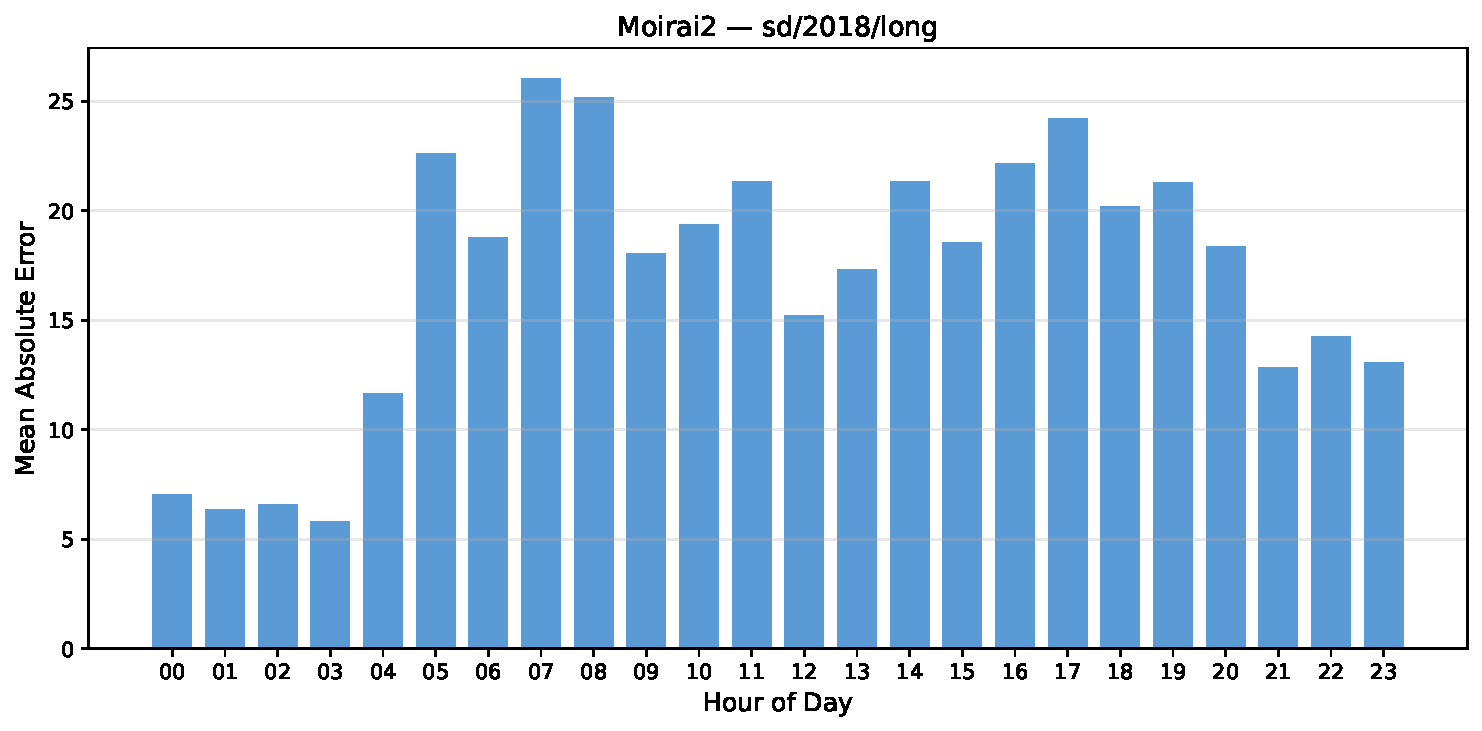
\includegraphics[width=\linewidth]{figs/hourly_mae_moirai2.pdf}
  \caption{\texttt{Moirai-2} (pretrained)}
\end{subfigure}
\hfill
\begin{subfigure}[t]{0.32\linewidth}
  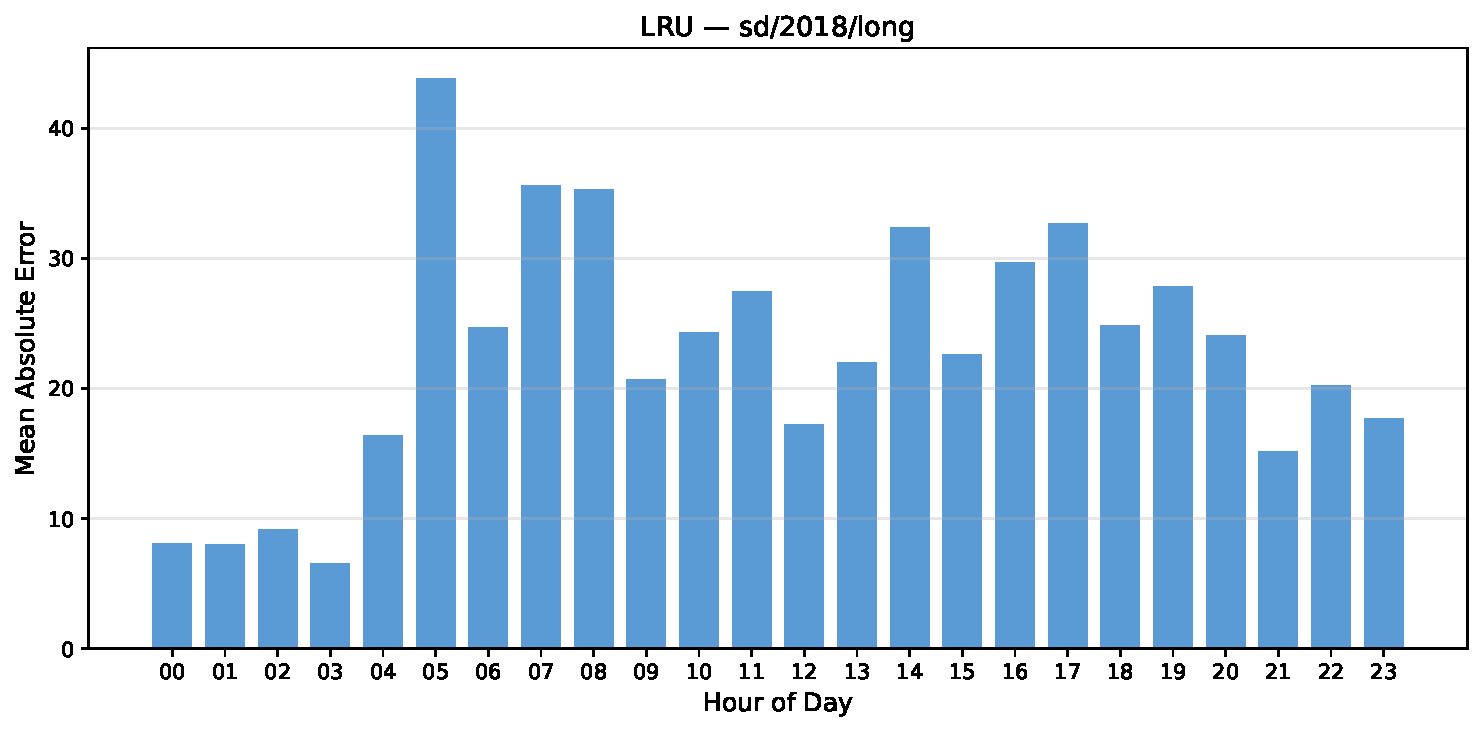
\includegraphics[width=\linewidth]{figs/hourly_mae_lru.pdf}
  \caption{\texttt{LRU} (state-space)}
\end{subfigure}
\hfill
\begin{subfigure}[t]{0.32\linewidth}
  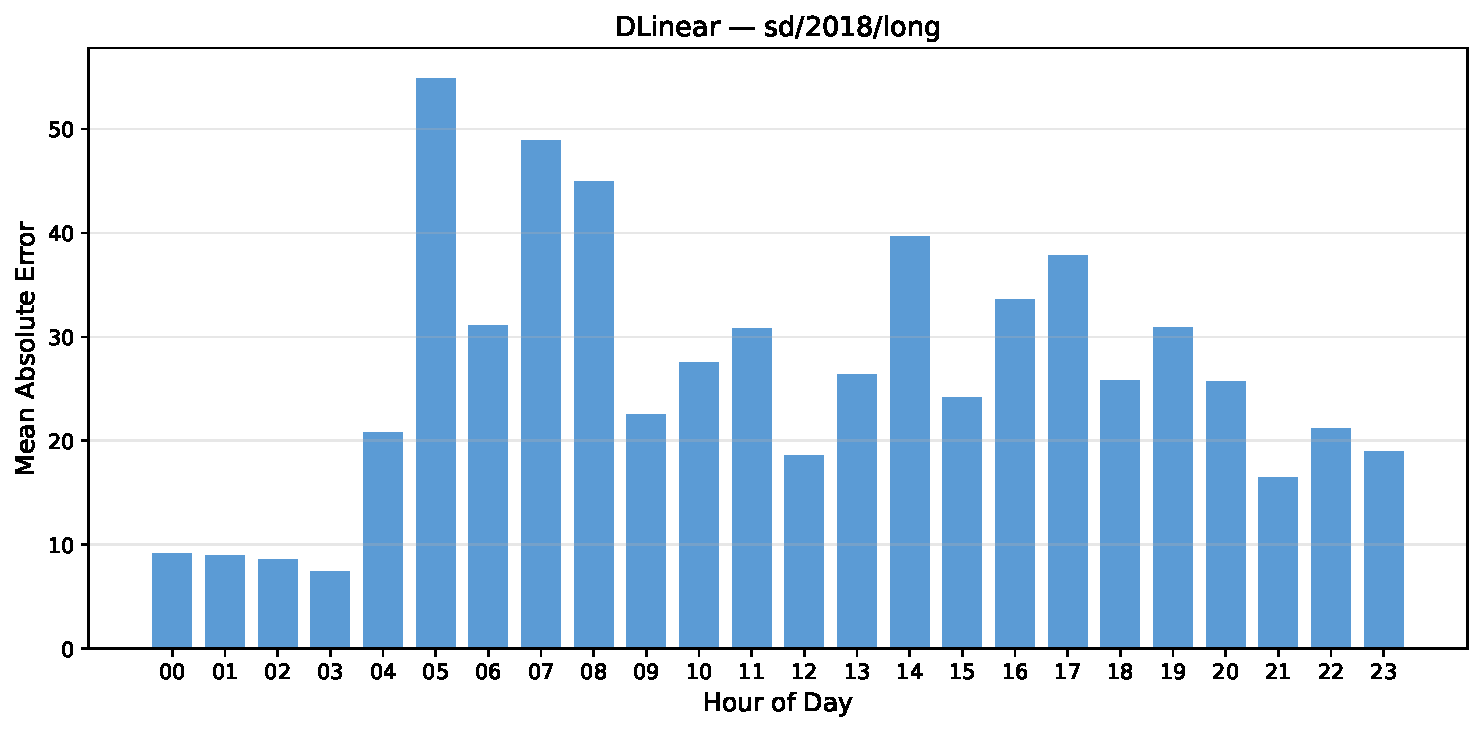
\includegraphics[width=\linewidth]{figs/hourly_mae_dlinear.pdf}
  \caption{\texttt{DLinear} (linear)}
\end{subfigure}
\\[4pt]
\begin{subfigure}[t]{0.32\linewidth}
  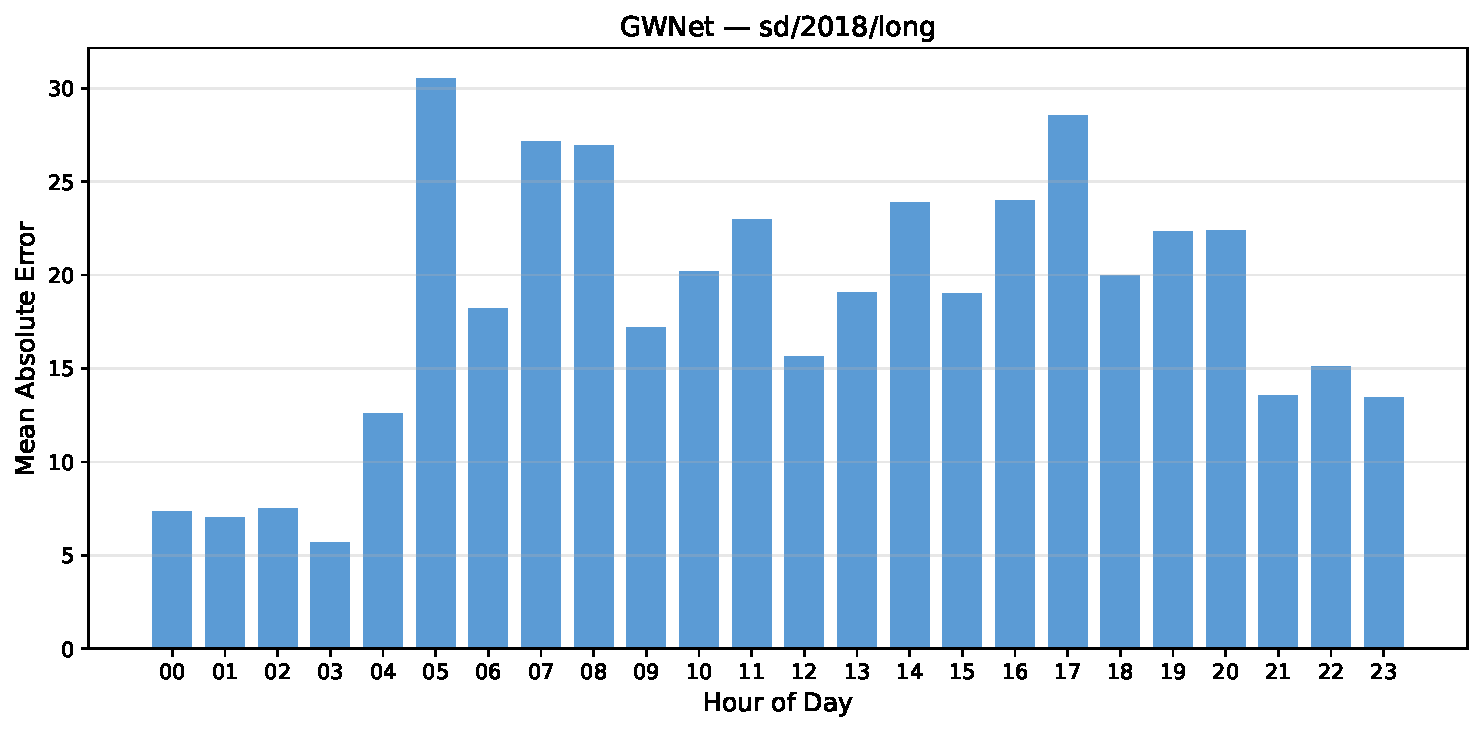
\includegraphics[width=\linewidth]{figs/hourly_mae_gwnet.pdf}
  \caption{\texttt{GWNET} (graph)}
\end{subfigure}
\hfill
\begin{subfigure}[t]{0.32\linewidth}
  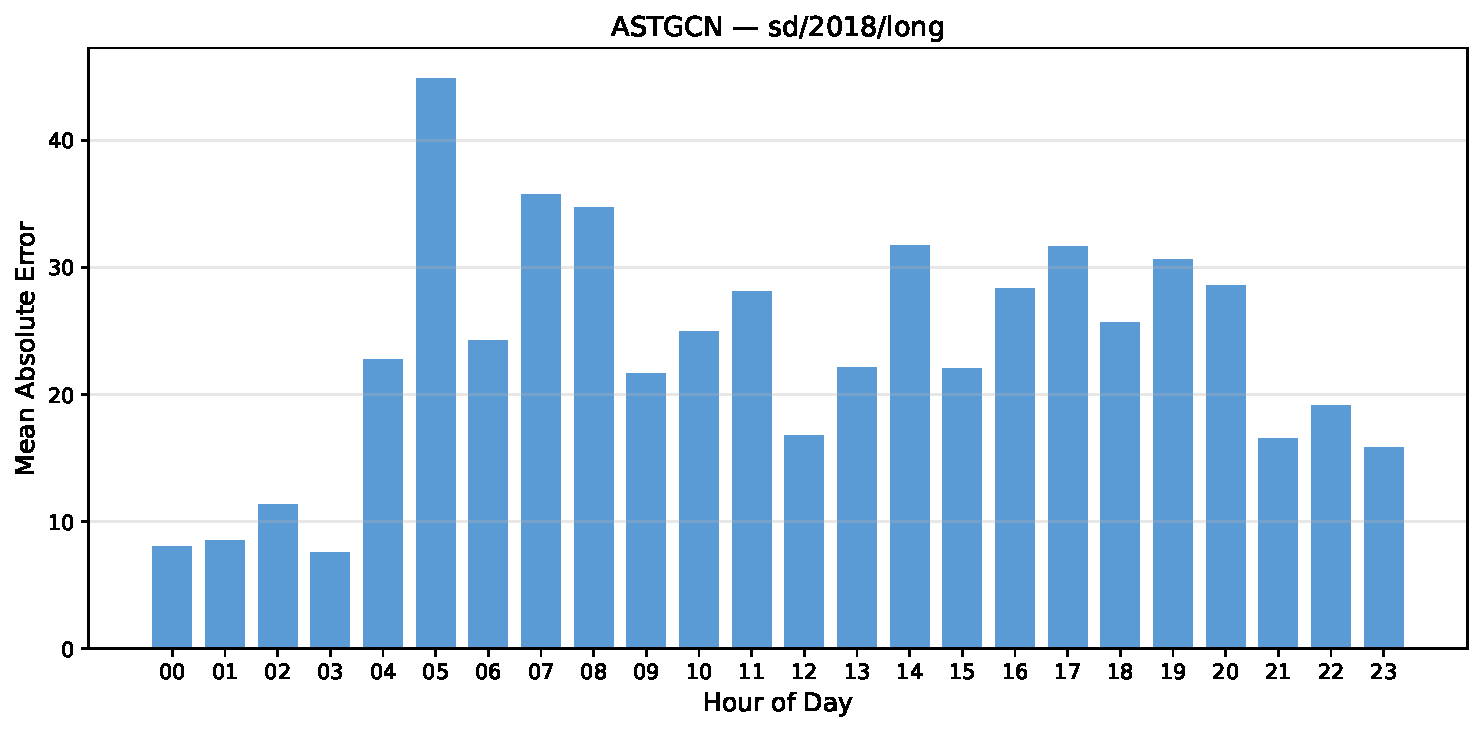
\includegraphics[width=\linewidth]{figs/hourly_mae_astgcn.pdf}
  \caption{\texttt{ASTGCN} (graph)}
\end{subfigure}
\hfill
\hspace{0.32\linewidth}
\caption{Hour-of-day MAE on SD~2018, averaged over all 716 sensors and the
twelve forecast steps, one representative per family. All five are scored on the
same 500 windows (2018-10-30 to 12-31), a wider span than the benchmark tables
so that every hour is sampled across two months; panels are comparable with each
other but not with the tables. All five bottom out at 03:00 and are hardest
through the morning ramp-up, but the peak hour is not shared: four of them peak
at 05:00 while \texttt{Moirai-2} peaks two hours later, at 07:00. At 05:00
itself---everyone else's worst hour---\texttt{Moirai-2} records 22.70 MAE
against 30.62 for \texttt{GWNET}, 43.97 for \texttt{LRU}, 45.02 for
\texttt{ASTGCN} and 55.03 for \texttt{DLinear}. This qualifies the main text's
reading, in which the morning spike is characteristic of recent-driven
foundation models: the spike is real for \texttt{Moirai-2} but arrives later and
is smaller than for any model it is contrasted with. \texttt{Moirai-2} also has
the flattest profile (worst-hour to best-hour ratio $4.4$, against $5.3$ for
\texttt{GWNET}, $5.9$ \texttt{ASTGCN}, $6.6$ \texttt{LRU}, $7.2$
\texttt{DLinear}) and the lowest error at 20 of the 24 hours; \texttt{GWNET}
takes the other four, each by less than $0.9$ MAE.}
\label{fig:app_hourly}
\end{figure*}

\begin{figure*}[t]
\centering
\begin{subfigure}[t]{\linewidth}
  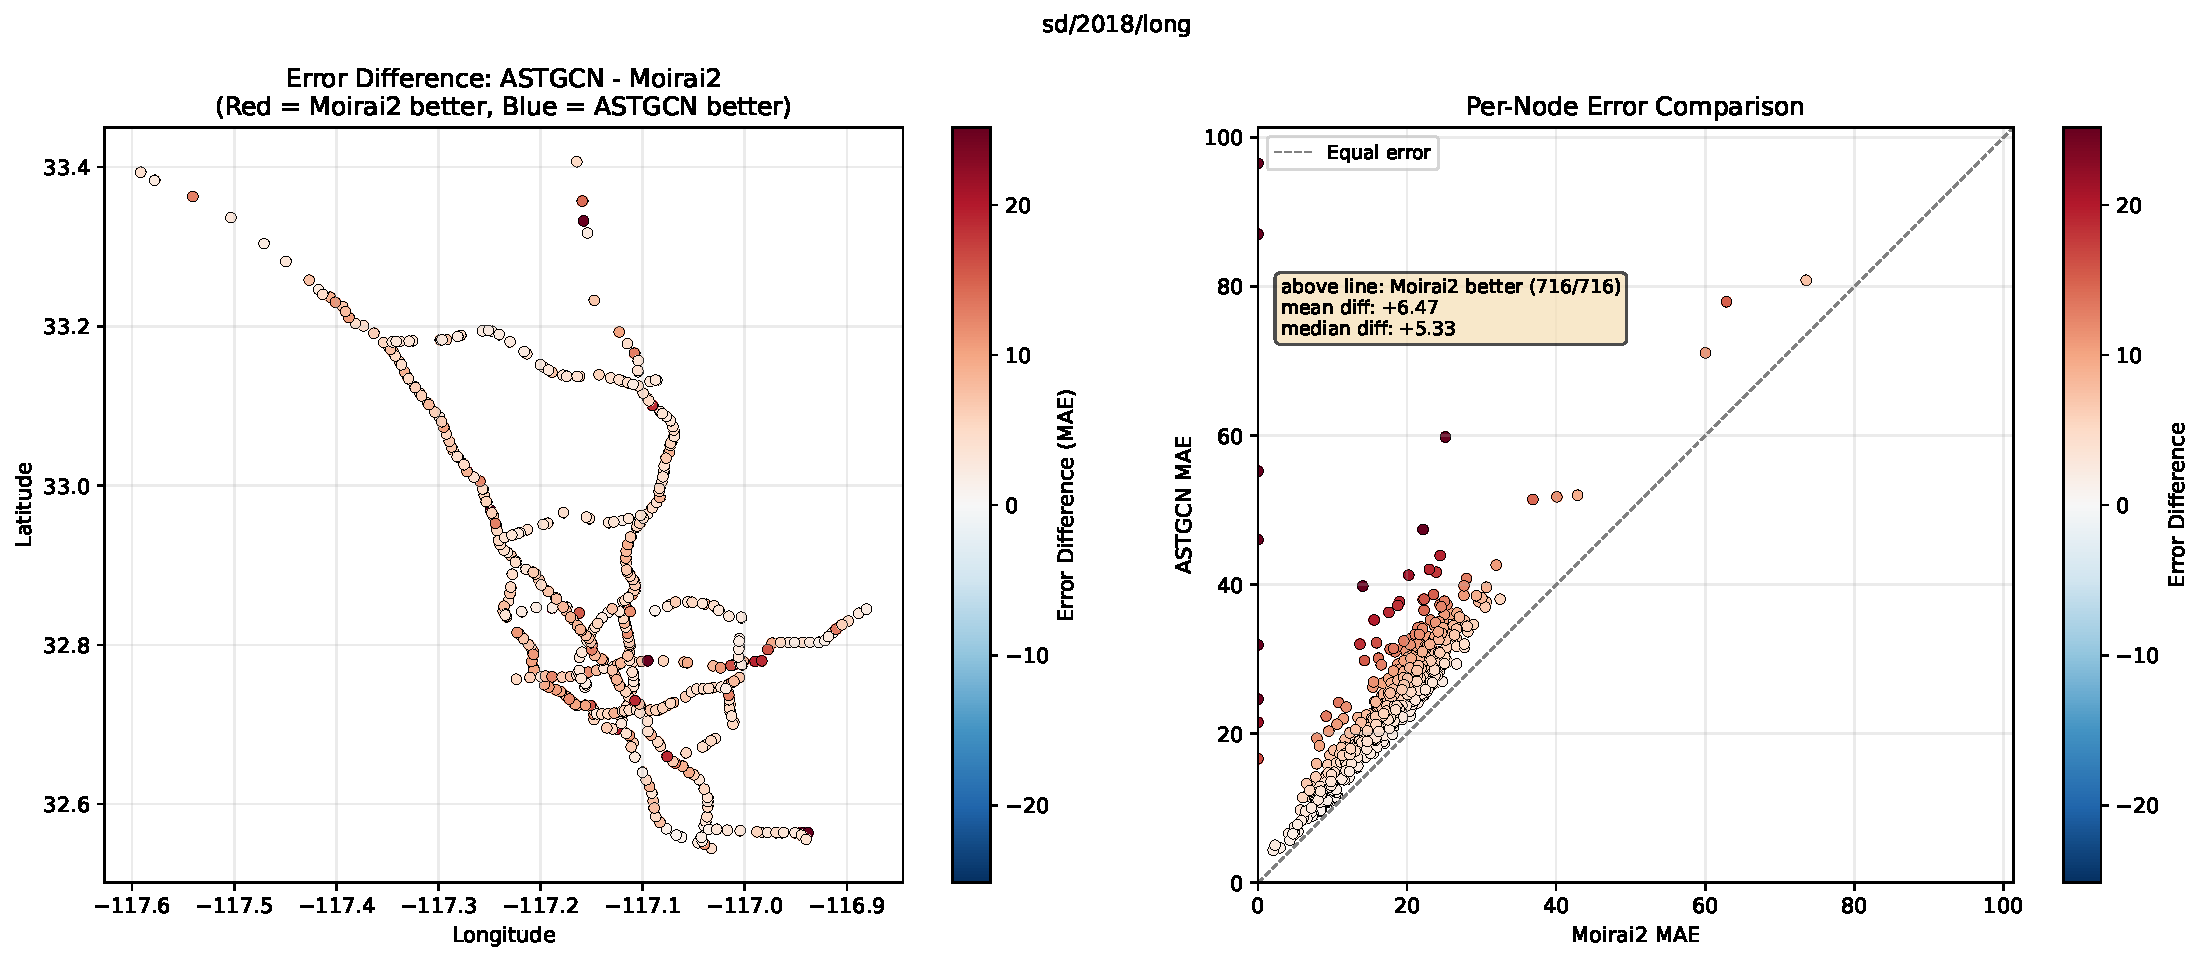
\includegraphics[width=\linewidth]{figs/node_error_astgcn_moirai2.pdf}
  \caption{\texttt{ASTGCN} against \texttt{Moirai-2}: the pretrained model wins
  on 716 of 716 sensors.}
\end{subfigure}
\\[6pt]
\begin{subfigure}[t]{\linewidth}
  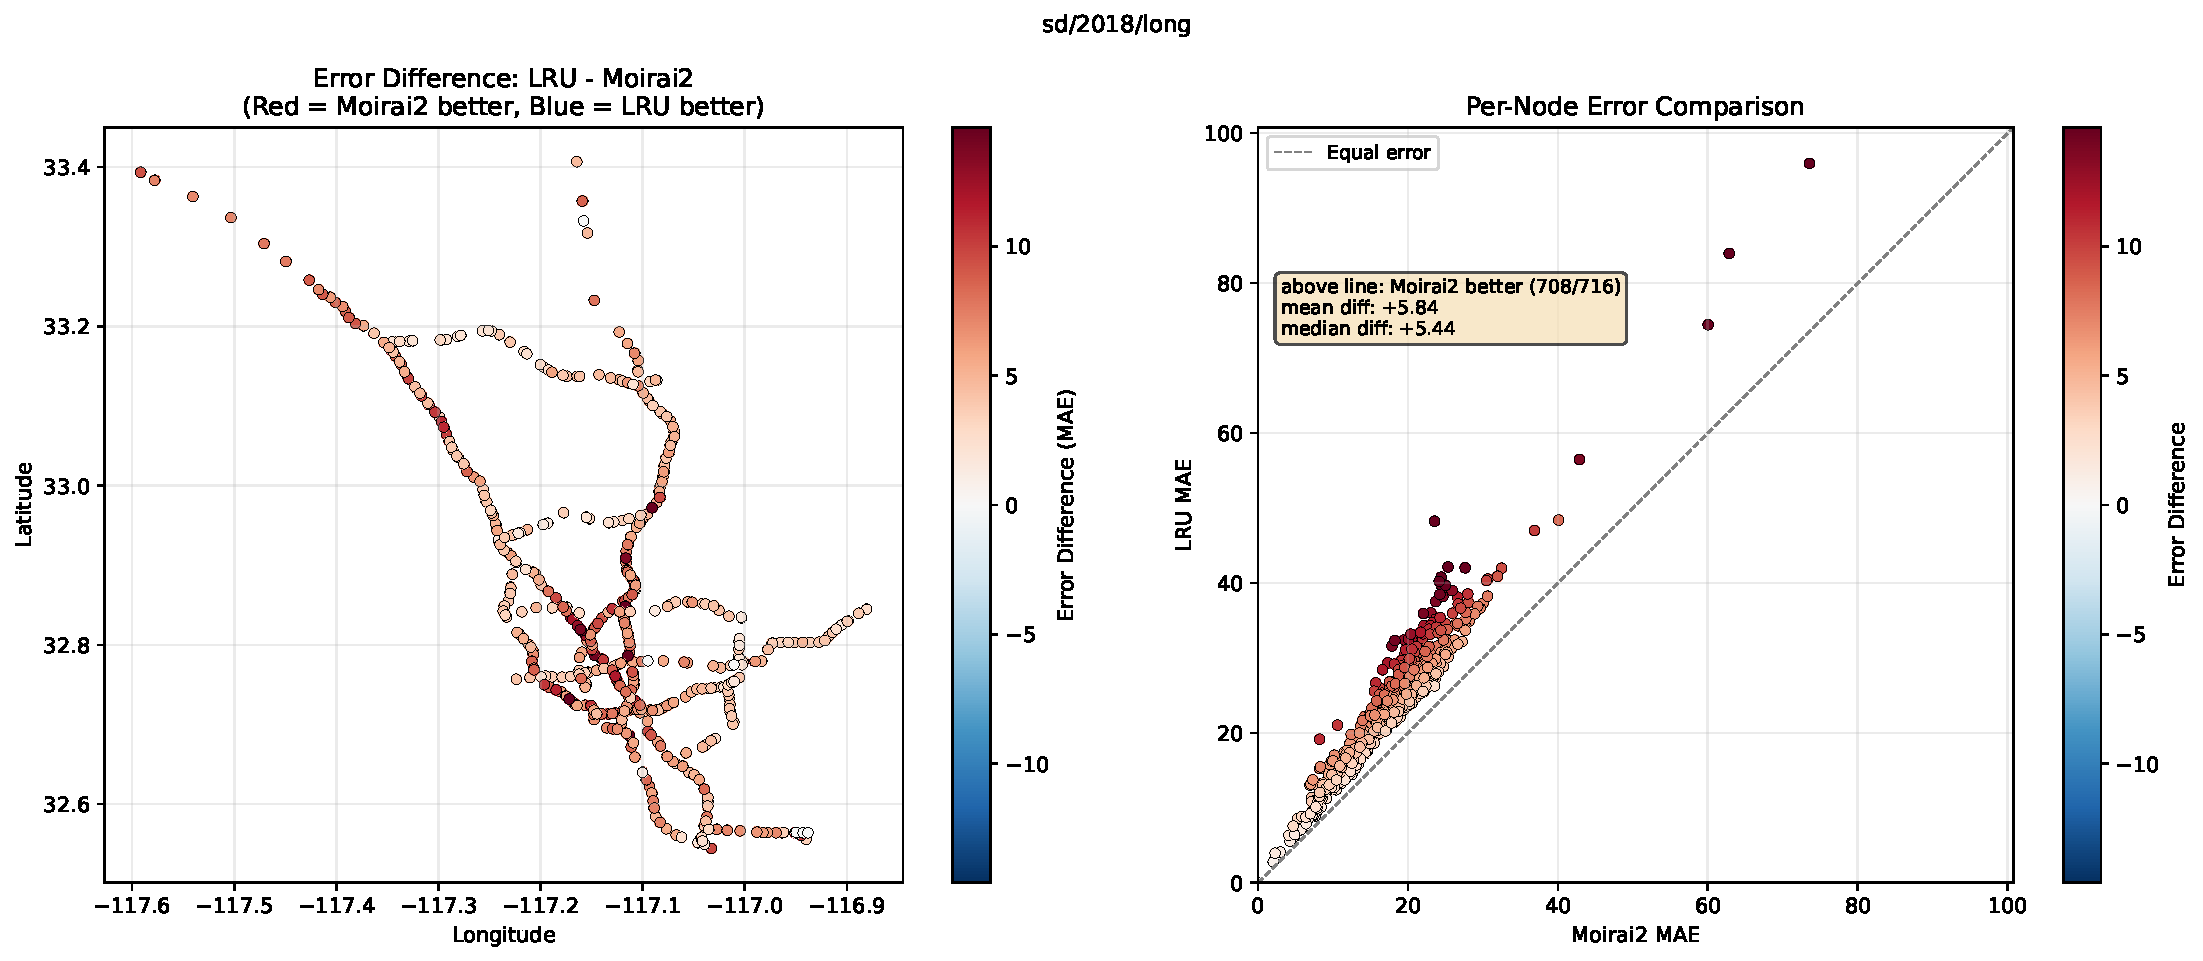
\includegraphics[width=\linewidth]{figs/node_error_lru_moirai2.pdf}
  \caption{\texttt{LRU} against \texttt{Moirai-2}: 708 of 716.}
\end{subfigure}
\caption{Per-sensor MAE on SD~2018 over all 716 sensors, same windows as
Figure~\ref{fig:app_hourly}. In each row, left is the spatial distribution of
the difference and right the per-sensor scatter against the $y=x$ line.
\emph{The pretrained model's advantage is uniform, not carried by outliers.}
\texttt{Moirai-2} (mean MAE $17.07$) is better than \texttt{ASTGCN} ($23.53$) on
\emph{every} sensor---a matched-pairs rank-biserial correlation of exactly
$+1.00$---and better than \texttt{LRU} ($22.90$) on $708$ of $716$ ($98.9\%$,
$r = +0.98$); both Wilcoxon signed-rank tests reject equality at
$p < 10^{-100}$. That this is a real property of the comparison and not of the
metric is clear from the same test applied to the two task-trained models:
\texttt{LRU} has a lower mean MAE than \texttt{ASTGCN} by $0.63$, but it wins
on only $330$ of $716$ sensors ($46.1\%$), the median difference runs the other
way, and Wilcoxon does not reject equality ($p = 0.092$). A mean gap can
therefore be uniform or an artifact of a few sensors, and on SD only the
pretrained model's is the former---consistent with
Section~\ref{app:extended:tables}, where SD is the one subset on which the
task-trained families do not separate.}
\label{fig:app_node}
\end{figure*}

\subsection{Information conditioning and the cost of full-graph inference}
\label{app:extended:asymmetry}

The two families are not conditioned on the same information. A spatiotemporal
GNN observes every sensor in the network simultaneously in a single forward
pass; the SSMs, linear forecasters and foundation models observe the history of
one sensor at a time and nothing else. Under identical data, splits, context
lengths and evaluation protocol, the graph models are strictly better informed
at prediction time.

That advantage does not appear in the results. On GBA and GLA, in both years,
the best graph-free model attains a lower MAE than \emph{every} executable graph
model at \emph{every} horizon---twelve comparisons out of twelve, with margins
that widen as the horizon grows (at $H{=}12$ on GLA~2019, 18.17 against 28.93).
This is not an artifact of pretraining scale: restricting the comparison to the
task-trained SSMs, which see the same training data under the same budget and
simply have no access to the adjacency, the same ordering holds at every horizon
on GLA and CA and at all but one on GBA. Whatever the graph contributes on these
networks, it is not being converted into accuracy.

The constraint is also unevenly distributed inside the family. The most accurate
graph model on SD, \texttt{DGCRN}, cannot be run on GLA or CA at all, and
\texttt{D2STGNN} cannot be run beyond SD---though the exclusion is not total,
since \texttt{AGCRN} places second on SD and executes everywhere. The cost of
full-graph inference is therefore not only that a forward pass is expensive and
needs a synchronized network-wide snapshot: the memory footprint removes some of
the family's most competitive members from consideration before accuracy is
measured, while per-series models remain available at every scale.

\subsection{Year-over-year stability}
\label{app:extended:years}

Ranking the shared methods by Avg MAE within each region and comparing 2018 to
2019 gives Spearman $\rho = 0.98$ on SD, $0.97$ on GBA, $0.95$ on GLA and
$0.87$ on CA. The family-level conclusions above are therefore not an artifact
of the year, which is the check the main text's single-year tables cannot
perform. Individual methods are much less stable than families---\texttt{STTN}
moves up four to eleven places depending on the subset, \texttt{AGCRN} up
eight on CA and \texttt{DSTAGNN} down six on GBA---but no such movement
changes which family leads. CA is the least stable subset
($\rho = 0.87$ against $0.95$--$0.98$ elsewhere), and
Section~\ref{app:extended:ca} locates the reason: the lag-feature regressors
and the ensembles built on them degrade far more between the two years than any
other family does. A single-year, single-region table is thus
adequate for choosing a \emph{family} and unreliable for ranking neighbours
within one, which is the paper's own thesis about fragmented protocols applied
to itself.

\begin{insightbox}
\textit{Takeaway:} Across four subsets and two years, pretrained foundation
models lead at every horizon rather than only at long ones---\texttt{Sundial} is
first in all eight cells (Wilcoxon $p = 0.0078$ against the best graph model in
each)---but the family is not uniform, and \texttt{TimesFM}, the largest model
evaluated, loses to the best state-space model everywhere. The graph models are
the only family conditioned on the whole network at inference time, yet on GBA
and GLA every executable one is beaten at every horizon by models that see a
single sensor, including task-trained SSMs that differ from them chiefly in
having no adjacency; on CA they trail the state-space models by $19$--$29\%$,
and their most accurate member cannot be run there at all. Spatial message passing is thus both
unrewarded at scale here and, for its strongest variants, unavailable---though
even with eight region-years the omnibus post-hoc test still cannot separate the
graph and pretrained families at $\alpha = 0.05$ (rank gap $2.75$ against a
critical difference of $2.85$), so the ordering is consistent rather than
individually certified.
\end{insightbox}
